%!TEX root = /Users/simo/Documents/PFC/memoria/memoria.tex
\section{Cuarto Ciclo} % (fold)
\label{sec:cuarto_ciclo}

Una vez se tiene el concepto de Grupo introducido en el sistema, está todo preparado para poder generar todo el sistema de permisos para la interfaz Javascript.

\subsection{Análisis de requisitos} % (fold)
\label{sub:análisis_de_requisitos}

\begin{itemize}
  \item Individualmente para cada documento, se debe poder definir una lista de usuarios y grupos que pueden \emph{participar} en este documento, definiendo para cada uno de estos si participan en calidad de espectador o de ponente. Un ponente puede \emph{dibujar} en la pizarra, los espectadores solo reciben los cambios hechos en las pizarra.
  \item Además, se debe poder hacer una pizarra pública, de forma que cualquier usuario pueda participar en forma de espectador.
\end{itemize}

% subsection análisis_de_requisitos (end)

\subsection{Diseño} % (fold)
\label{sub:diseño}

El concepto de permisos es semejante al concepto de invitaciones, siendo la única diferencia que no es algo que se pueda rechazar. El creador del documento puede añadir o quitar conexiones entre un documento y un usuario o grupo, que además deberá constatar si es en forma de ponente o de observador, necesitando pues, una clase asociativa.

\begin{figure}[h!]
\centering
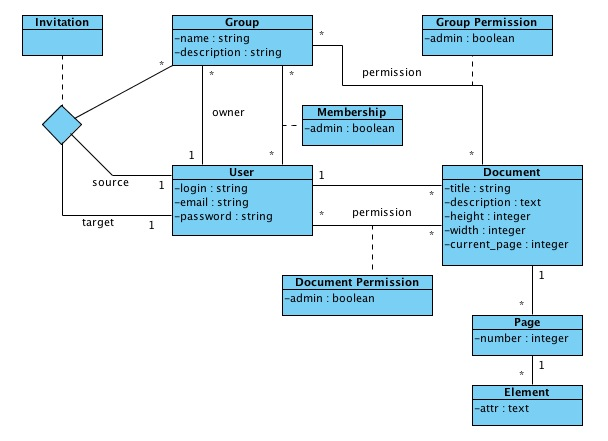
\includegraphics[width=14cm]{uml4.png}
\caption{Clases del dominio, 4º ciclo}\label{fig:uml4}
\end{figure}

Y por lo tanto, normalizado:

\begin{figure}[h!]
\centering
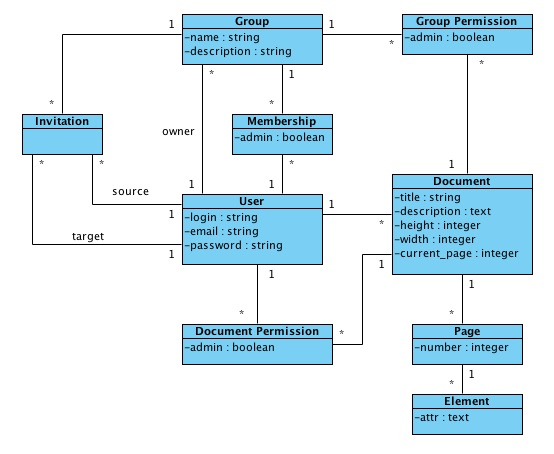
\includegraphics[width=14cm]{uml4n.png}
\caption{Clases del dominio, 4º ciclo, diagrama normalizado}\label{fig:uml4n}
\end{figure}

% subsection diseño (end)

\subsection{Implementación} % (fold)
\label{sub:implementación}

De nuevo, traducir estas dos nuevas clases a modelos de Rails es sencillo. El proceso de integrar estas nuevas funcionalidades en el sistema, es más un problema de encontrar una interfaz adecuada para todas estas operaciones, que de implementación de los controladores.

Finalmente el diagrama de clases se ha convertido en algo más grande, e incluso con las facilidades que ofrece Rails para manejar todas estas relaciones, es importante mantener todo bien organizado. Se considera una buena práctica tener la mayor parte del código implementada en los modelos. Esto es así puesto que una función implementada en un modelo siempre es reutilizable, y poniéndose un límite de unas 10 líneas de código en cada función del controlador, hace que se tenga en todo momento unas acciones bien claras y definidas, y por lo tanto, de muy fácil modificación en futuras iteraciones.

Así pues, lo más fácil es implementar funciones como las siguientes:

\begin{Verbatim}[commandchars=@\[\]]
  document@PYbf[.]can_be_seen_by?(user)
  document@PYbf[.]can_be_edited_by?(user)
  document@PYbf[.]can_be_deleted_by?(user)
  user@PYbf[.]all_accessible_documents
  user@PYbf[.]invite(user,group)
  group@PYbf[.]is_member?(user)
  group@PYbf[.]is_admin?(user)
  group@PYbf[.]is_owner?(user)
  group@PYbf[.]add_user(user)
  group@PYbf[.]promote(user)
  group@PYbf[.]unpromote(user)
\end{Verbatim}


%\begin{verbatim}
%  document.can_be_seen_by?(user)
%  document.can_be_edited_by?(user)
%  document.can_be_deleted_by?(user)
%  user.all_accessible_documents
%  user.invite(user,group)
%  group.is_member?(user)
%  group.is_admin?(user)
%  group.is_owner?(user)
%  group.add_user(user)
%  group.promote(user)
%  group.unpromote(user)
%\end{verbatim}

Todas son completamente autoexplicativas gracias a sus nombres, y contribuyen a que los controladores simplifiquen la mayoría de su código dejando solamente las líneas esenciales para que cualquier programador pueda saber de un vistazo qué hace este controlador.

Teniendo estas funciones implementadas, modificar las cuatro acciones de comunicación con el motor para tenerlas en cuenta, no necesita más que una línea extra.

% subsection implementación (end)

% section cuarto_ciclo (end)